\documentclass[border=10pt]{standalone}

\usepackage{tikz}
\usepackage{tikzsymbols}
\usetikzlibrary{calc,patterns,shapes.geometric}

\def\centerarc[#1](#2)(#3:#4:#5){\draw[#1] ($(#2)+({#5*cos(#3)},{#5*sin(#3)})$) arc (#3:#4:#5);}

\begin{document}
	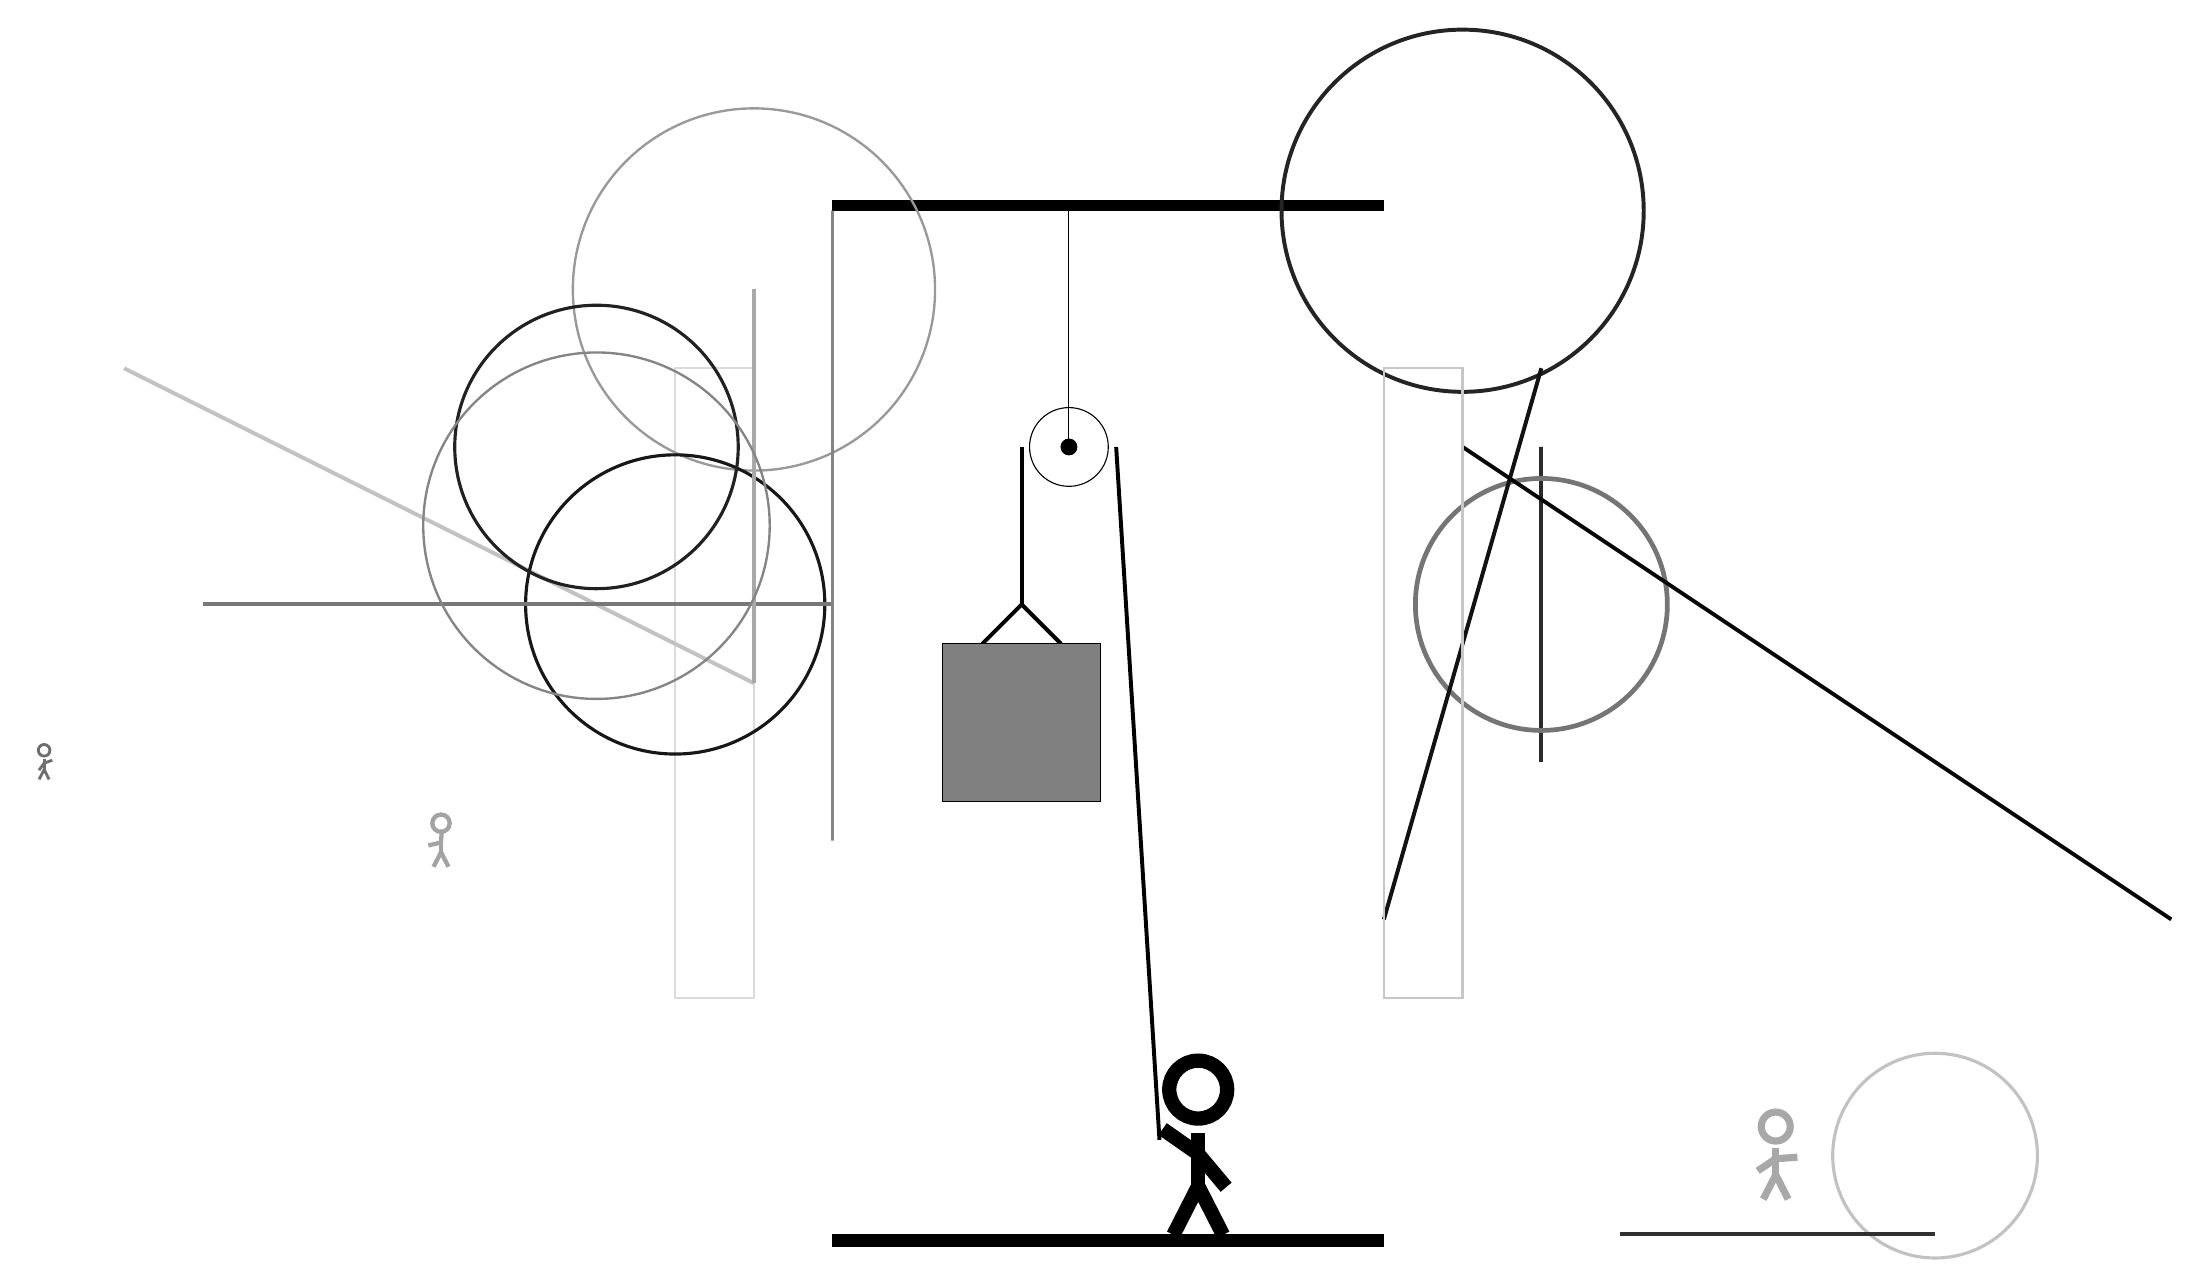
\begin{tikzpicture}
		%%%%% START %%%%%
		
		\draw[fill=black] (-2, 10) rectangle (5, 10.125);
		
		\draw (1, 7) circle (0.5);
		\draw[fill=black] (1, 7) circle (0.1);
		\draw (1, 10) -- (1, 7);
		
		\draw[line width=0.5mm] (-0.1, 4.5) -- (0.4, 5.0) -- (0.9, 4.5);
		\draw[fill=black!50] (-0.6, 4.5) rectangle (1.4, 2.5);
		
		\draw[line width=0.5mm] (0.4, 7) -- (0.4, 5.0);
		\centerarc[line width=0.5mm](1, 7)(0:180:0.6);
		\draw[line width=0.5mm](1.6, 7) -- (2.15, -1.8);
		
		\node at (2.6, -1.9) {\Strichmaxerl[10][-35][-50]};
		
		\draw [line width=0.5mm, color=black!86](6, 10) circle (2.3);
		
		\draw[line width=0.5mm, color=black!83] (7, 7) rectangle (7, 3);
		\draw[line width=0.3mm, color=black!14] (-3, 8) rectangle (-4, 0);
		\draw[line width=0.5mm, color=black!24](-3, 4) -- (-11, 8);
		\draw [line width=0.6mm, color=black!54](7, 5) circle (1.6);
		\draw [line width=0.4mm, color=black!24](12, -2) circle (1.3);
		
		\draw [line width=0.3mm, color=black!40](-3, 9) circle (2.3);
		
		\draw [line width=0.4mm, color=black!91](-4, 5) circle (1.9);
		\node[line width=0.7mm, color=black!57] at (-12, 3) {\Strichmaxerl[2][54][20]};
		\draw[line width=0.5mm, color=black!81](8, -3) -- (12, -3);
		\node[line width=0.4mm, color=black!34] at (10, -2) {\Strichmaxerl[5][34][4]};
		\draw [line width=0.4mm, color=black!87](-5, 7) circle (1.8);
		\draw[line width=0.5mm, color=black!53](-2, 5) -- (-10, 5);
		\node[line width=0.6mm, color=black!36] at (-7, 2) {\Strichmaxerl[3][13][86]};
		\draw[line width=0.5mm, color=black!34](-3, 9) -- (-3, 4);
		\draw[line width=0.4mm, color=black!48] (-2, 10) rectangle (-2, 2);
		
		\draw[line width=0.5mm, color=black!93](5, 1) -- (7, 8);
		\draw [line width=0.3mm, color=black!48](-5, 6) circle (2.2);
		\draw[line width=0.5mm, color=black!97](6, 7) -- (15, 1);
		
		\draw[line width=0.3mm, color=black!22] (5, 0) rectangle (6, 8);
		
		\draw[fill=black] (-2, -3) rectangle (5, -3.15);
		
		%%%%% END %%%%%
	\end{tikzpicture}
\end{document}